\documentclass[tikz,border=10pt]{standalone}
% Shared look for every TikZ diagram. Load with % Shared look for every TikZ diagram. Load with % Shared look for every TikZ diagram. Load with \input{../../tools/tikz-style.tex}
\usepackage[T1]{fontenc}
\usepackage{lmodern}
\renewcommand{\sfdefault}{lmr}  % diagrams use the same serif as the text
\usetikzlibrary{arrows.meta, positioning, shapes.geometric, calc, fit, backgrounds}
\definecolor{cblue}{HTML}{4C78A8}
\definecolor{corange}{HTML}{F58518}
\definecolor{cgreen}{HTML}{54A24B}
\definecolor{cred}{HTML}{E45756}
\definecolor{cpurple}{HTML}{B279A2}
\definecolor{cgrey}{HTML}{6B6B6B}
\tikzset{
  every picture/.style={font=\sffamily, line width=1.2pt},
  box/.style={draw=#1, fill=#1!12, rounded corners=4pt, align=center, inner sep=7pt, minimum height=1.1cm},
  box/.default=cgrey,
  arrow/.style={-{Stealth[length=3mm]}, draw=cgrey, line width=1.4pt},
  title/.style={font=\sffamily\bfseries\Large},
  note/.style={font=\sffamily\small, text=cgrey, align=center},
}
\AtBeginDocument{\hyphenpenalty=10000 \exhyphenpenalty=10000}

\usepackage[T1]{fontenc}
\usepackage{lmodern}
\renewcommand{\sfdefault}{lmr}  % diagrams use the same serif as the text
\usetikzlibrary{arrows.meta, positioning, shapes.geometric, calc, fit, backgrounds}
\definecolor{cblue}{HTML}{4C78A8}
\definecolor{corange}{HTML}{F58518}
\definecolor{cgreen}{HTML}{54A24B}
\definecolor{cred}{HTML}{E45756}
\definecolor{cpurple}{HTML}{B279A2}
\definecolor{cgrey}{HTML}{6B6B6B}
\tikzset{
  every picture/.style={font=\sffamily, line width=1.2pt},
  box/.style={draw=#1, fill=#1!12, rounded corners=4pt, align=center, inner sep=7pt, minimum height=1.1cm},
  box/.default=cgrey,
  arrow/.style={-{Stealth[length=3mm]}, draw=cgrey, line width=1.4pt},
  title/.style={font=\sffamily\bfseries\Large},
  note/.style={font=\sffamily\small, text=cgrey, align=center},
}
\AtBeginDocument{\hyphenpenalty=10000 \exhyphenpenalty=10000}

\usepackage[T1]{fontenc}
\usepackage{lmodern}
\renewcommand{\sfdefault}{lmr}  % diagrams use the same serif as the text
\usetikzlibrary{arrows.meta, positioning, shapes.geometric, calc, fit, backgrounds}
\definecolor{cblue}{HTML}{4C78A8}
\definecolor{corange}{HTML}{F58518}
\definecolor{cgreen}{HTML}{54A24B}
\definecolor{cred}{HTML}{E45756}
\definecolor{cpurple}{HTML}{B279A2}
\definecolor{cgrey}{HTML}{6B6B6B}
\tikzset{
  every picture/.style={font=\sffamily, line width=1.2pt},
  box/.style={draw=#1, fill=#1!12, rounded corners=4pt, align=center, inner sep=7pt, minimum height=1.1cm},
  box/.default=cgrey,
  arrow/.style={-{Stealth[length=3mm]}, draw=cgrey, line width=1.4pt},
  title/.style={font=\sffamily\bfseries\Large},
  note/.style={font=\sffamily\small, text=cgrey, align=center},
}
\AtBeginDocument{\hyphenpenalty=10000 \exhyphenpenalty=10000}

\begin{document}
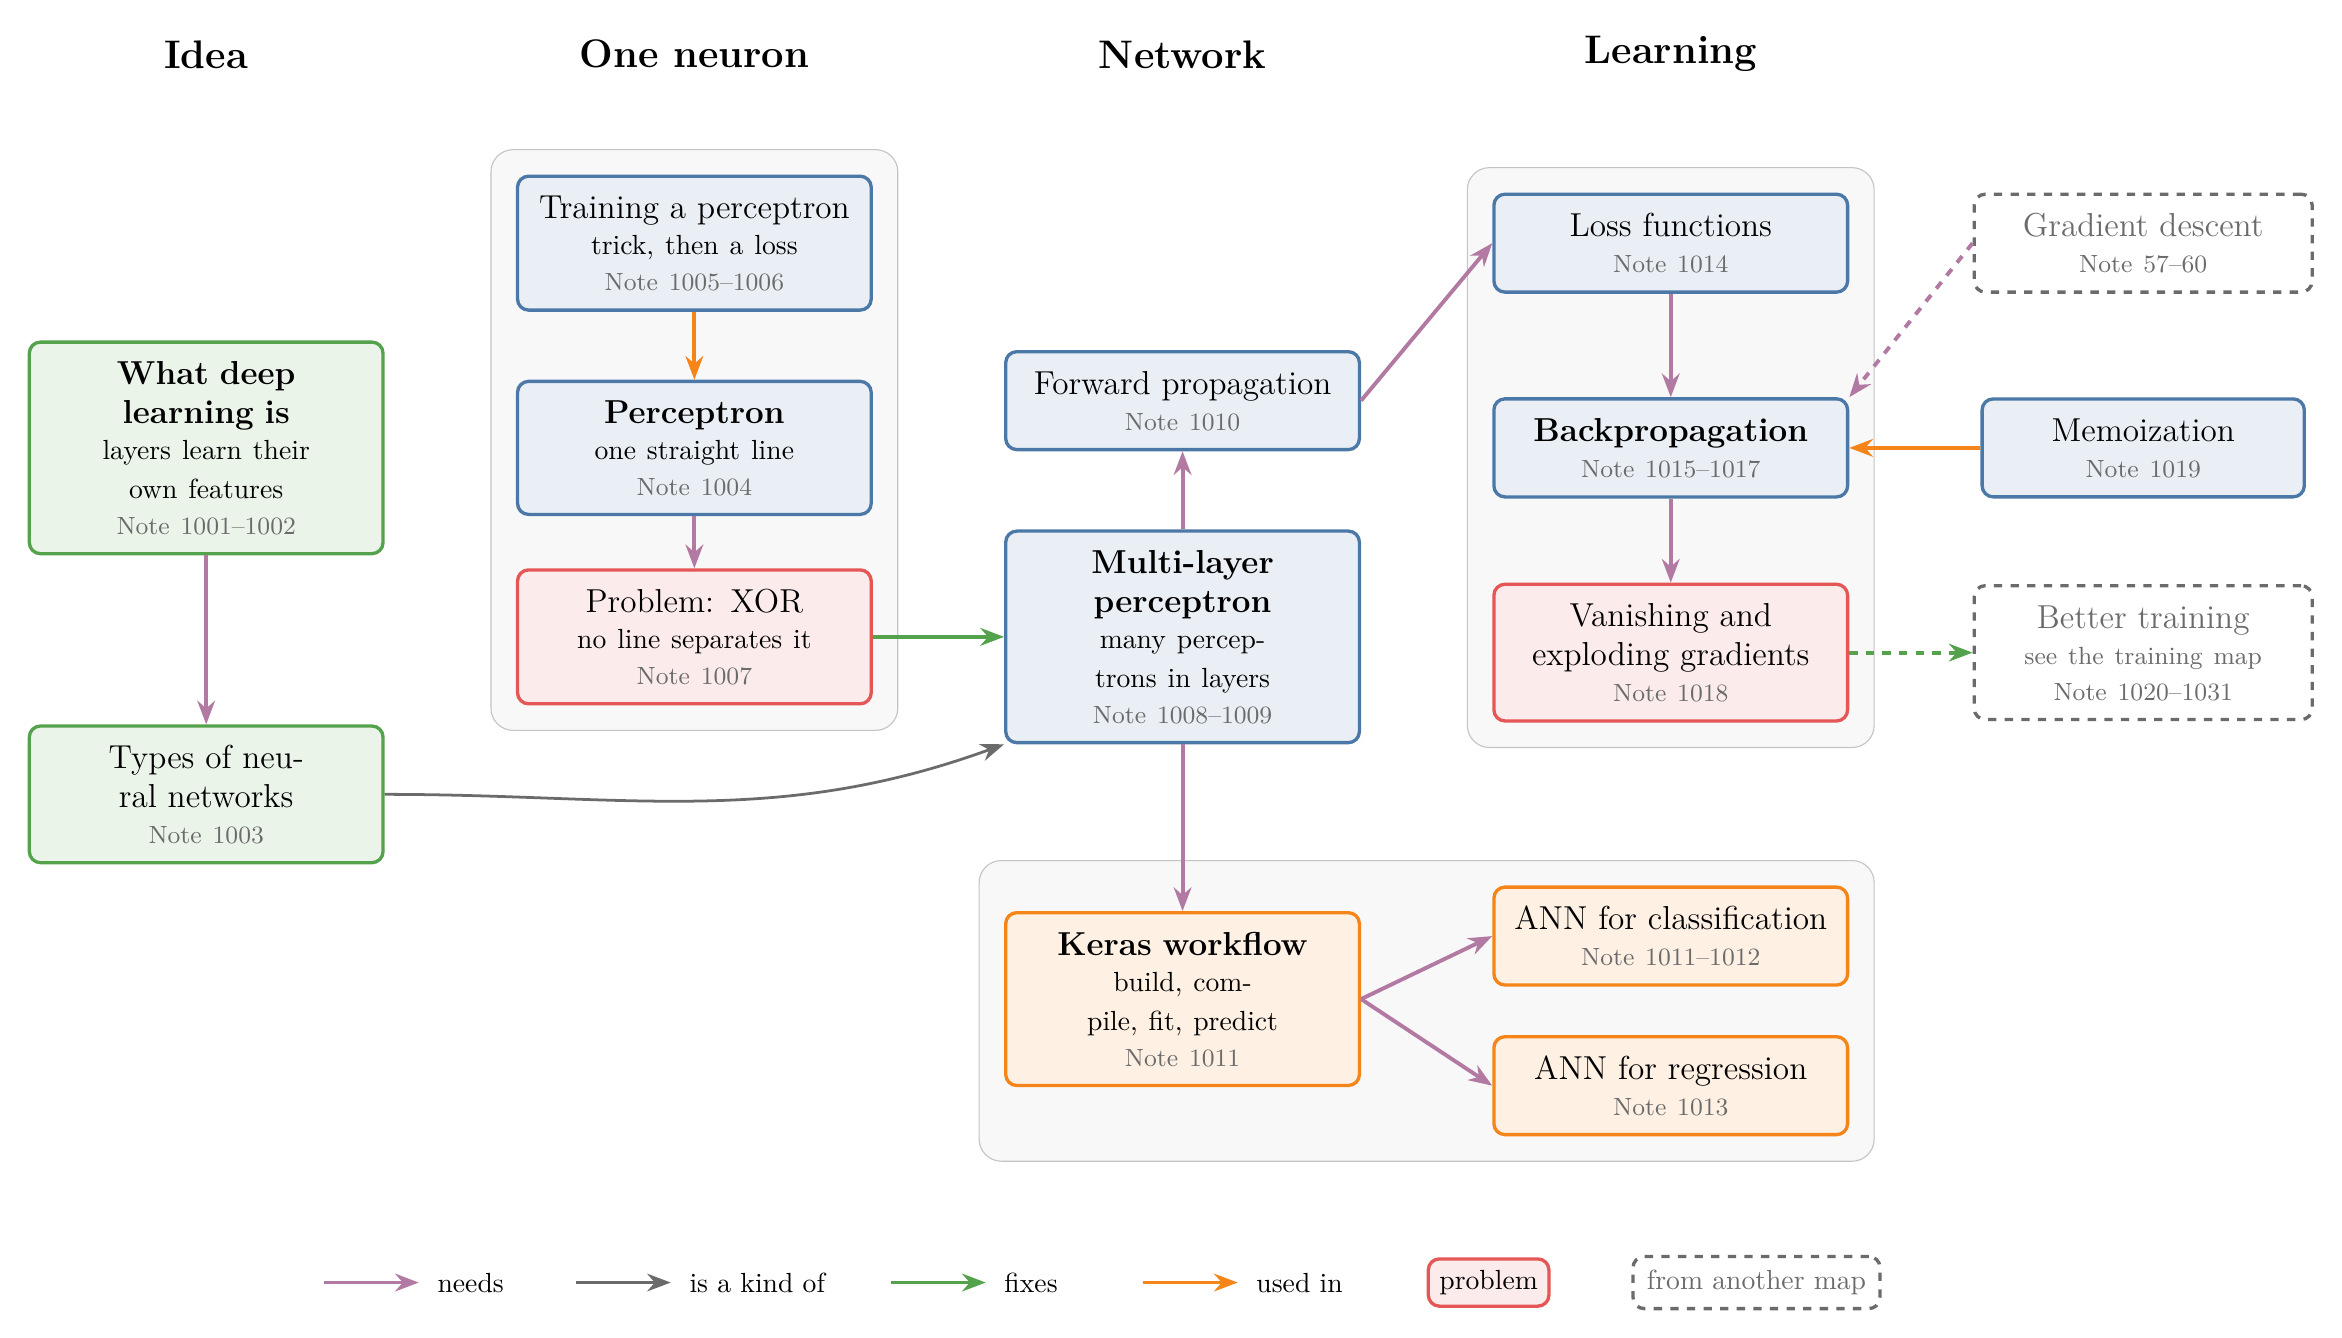
\begin{tikzpicture}[
    every node/.append style={font=\sffamily\large},
    con/.style={box=cblue, text width=4.0cm},
    prob/.style={box=cred, text width=4.0cm},
    prev/.style={draw=cgrey, dashed, rounded corners=4pt, align=center, inner sep=7pt, text=cgrey, text width=3.8cm, minimum height=1.1cm},
    group/.style={draw=cgrey!40, fill=cgrey!5, rounded corners=8pt, inner sep=9pt},
    kind/.style={arrow, draw=cgrey, line width=1pt},
    needs/.style={arrow, draw=cpurple},
    fixes/.style={arrow, draw=cgreen},
    usedin/.style={arrow, draw=corange},
  ]
  \newcommand{\nt}[1]{\\[-1pt]{\small\color{cgrey}Note #1}}
  \newcommand{\sub}[1]{\\[-1pt]{\normalsize #1}}
  \node[title] at (0,10.0) {Idea};
  \node[title] at (6.2,10.0) {One neuron};
  \node[title] at (12.4,10.0) {Network};
  \node[title] at (18.6,10.0) {Learning};

  % idea
  \node[box=cgreen, text width=4.0cm] (dl) at (0,5.0) {\textbf{What deep learning is}\sub{layers learn their own features}\nt{1001--1002}};
  \node[box=cgreen, text width=4.0cm] (types) at (0,0.6) {Types of neural networks\nt{1003}};
  \draw[needs] (dl) -- (types);

  % one neuron
  \node[con] (train) at (6.2,7.6) {Training a perceptron\sub{trick, then a loss}\nt{1005--1006}};
  \node[con] (perc) at (6.2,5.0) {\textbf{Perceptron}\sub{one straight line}\nt{1004}};
  \node[prob] (xor) at (6.2,2.6) {Problem: XOR\sub{no line separates it}\nt{1007}};
  \begin{scope}[on background layer]
    \node[group, fit=(train) (perc) (xor)] {};
  \end{scope}
  \draw[usedin] (train) -- (perc);
  \draw[needs] (perc) -- (xor);

  % network
  \node[con] (mlp) at (12.4,2.6) {\textbf{Multi-layer perceptron}\sub{many perceptrons in layers}\nt{1008--1009}};
  \node[con] (fwd) at (12.4,5.6) {Forward propagation\nt{1010}};
  \draw[fixes] (xor) -- (mlp);
  \draw[needs] (mlp) -- (fwd);
  \draw[kind] (types.east) to[out=0, in=200] (mlp.south west);

  % learning
  \node[con] (loss) at (18.6,7.6) {Loss functions\nt{1014}};
  \node[con] (bp) at (18.6,5.0) {\textbf{Backpropagation}\nt{1015--1017}};
  \node[prob] (van) at (18.6,2.4) {Vanishing and exploding gradients\nt{1018}};
  \begin{scope}[on background layer]
    \node[group, fit=(loss) (bp) (van)] {};
  \end{scope}
  \draw[needs] (fwd.east) -- (loss.west);
  \draw[needs] (loss) -- (bp);
  \draw[needs] (bp) -- (van);
  \node[con, text width=3.6cm] (memo) at (24.6,5.0) {Memoization\nt{1019}};
  \draw[usedin] (memo) -- (bp);
  \node[prev] (gd) at (24.6,7.6) {Gradient descent\nt{57--60}};
  \draw[needs, dashed] (gd.west) -- (bp.north east);
  \node[prev] (next) at (24.6,2.4) {Better training\\[-1pt]{\small see the training map}\nt{1020--1031}};
  \draw[fixes, dashed] (van) -- (next);

  % in code
  \node[box=corange, text width=4.0cm] (keras) at (12.4,-2.0) {\textbf{Keras workflow}\sub{build, compile, fit, predict}\nt{1011}};
  \node[box=corange, text width=4.0cm] (cls) at (18.6,-1.2) {ANN for classification\nt{1011--1012}};
  \node[box=corange, text width=4.0cm] (reg) at (18.6,-3.1) {ANN for regression\nt{1013}};
  \begin{scope}[on background layer]
    \node[group, fit=(keras) (cls) (reg)] {};
  \end{scope}
  \draw[needs] (mlp) -- (keras);
  \draw[needs] (keras.east) -- (cls.west);
  \draw[needs] (keras.east) -- (reg.west);

  % legend
  \begin{scope}[shift={(1.5,-5.6)}, every node/.style={font=\sffamily, anchor=west}]
    \draw[needs] (0,0) -- (1.2,0);      \node at (1.3,0) {needs};
    \draw[kind] (3.2,0) -- (4.4,0);     \node at (4.5,0) {is a kind of};
    \draw[fixes] (7.2,0) -- (8.4,0);    \node at (8.5,0) {fixes};
    \draw[usedin] (10.4,0) -- (11.6,0); \node at (11.7,0) {used in};
    \node[box=cred, minimum height=0.6cm, inner sep=4pt, anchor=west] at (14.0,0) {problem};
    \node[draw=cgrey, dashed, rounded corners=4pt, inner sep=5pt, text=cgrey, anchor=west] at (16.6,0) {from another map};
  \end{scope}
\end{tikzpicture}
\end{document}
